\phantomsection
\part*{論理と証明}
\phantomsection
\section{論理}
\phantomsection
\subsection{命題論理\index{めいだいろんり@命題論理}}

命題論理では,命題を結合するために記号を用いる.代表的な論理記号を列挙してみよう:

\begin{table}[ht]
  \centering
  \caption{命題論理の記号}
  \begin{tabular}{c|c}
    \hline
    記号                & 意味                       \\
    \hline
    $\land$           & かつ(論理積\index{ろんりせき@論理積}) \\
    $\lor$            & または(論理和\index{ろんりわ@論理和}) \\
    $\lnot$           & 否定\index{ひてい@否定}         \\
    $\to$             & ならば(含意\index{がんい@含意})    \\
    $\leftrightarrow$ & 同値 \index{どうち@同値} \\
    \hline
  \end{tabular}
\end{table}

これらの論理記号を用いて,命題を結合し,複雑な論理式を構成することができる.
以下に,基本的な命題の真理値表を載せよう.

\begin{table}[htbp]
  \begin{center}
    \begin{tabular}{c}

      \begin{minipage}{0.3\hsize}
        \begin{center}
          \caption{論理和(積)の真理値表}
          \label{fig:論理和(積)の真理値表}
          \begin{tabular}{|c|c|c|c|} \hline
            $P$           & $Q$          & $P \land Q$   & $P \lor Q$    \\ \hline
            $\mathrm{T}$  & $\mathrm{T}$ & $\mathrm{T}$  & $\mathrm{T}$  \\ \hline
            $\mathrm{T} $ & $\mathrm{F}$ & $\mathrm{F}$  & $\mathrm{T}$  \\ \hline
            $\mathrm{F} $ & $\mathrm{T}$ & $\mathrm{F} $ & $\mathrm{T}$  \\  \hline
            $\mathrm{F}$  & $\mathrm{F}$ & $\mathrm{F}$  & $\mathrm{F} $ \\ \hline
          \end{tabular}
        \end{center}
      \end{minipage}

      \begin{minipage}{0.3\hsize}
        \begin{center}
          \caption{否定命題の真理値表}
          \label{fig:否定命題の真理値表}
          \begin{tabular}{|c|c|} \hline
            $P $         & $\lnot P$    \\ \hline
            $\mathrm{T}$ & $\mathrm{F}$ \\ \hline
            $\mathrm{F}$ & $\mathrm{T}$ \\\hline
          \end{tabular}
        \end{center}
      \end{minipage}

      \begin{minipage}{0.3\hsize}
        \begin{center}
          \caption{恒真命題と矛盾命題の真理値表}
          \label{fig:恒真命題と矛盾命題の真理値表}
          \begin{tabular}{|c|c|c|c|} \hline
            $ P$          & $\lnot P$     & $ P \lor \lnot P $ & $P \land \lnot P$ \\ \hline
            $\mathrm{T} $ & $\mathrm{F} $ & $\mathrm{T}$       & $\mathrm{F}$      \\ \hline
            $\mathrm{F} $ & $\mathrm{T}$  & $\mathrm{T}$       & $\mathrm{F}$      \\\hline
          \end{tabular}
        \end{center}
      \end{minipage}
    \end{tabular}
  \end{center}
\end{table}
\begin{table}[htbp]
  \begin{center}
    \begin{tabular}{c}
      \begin{minipage}{0.5\hsize}
        \begin{center}
          \caption{「含意」の真理値表}
          \label{fig:「含意」の真理値表}
          \begin{tabular}{|c|c|c|} \hline
            $P$           & $Q$          & $P \to Q$      \\ \hline
            $\mathrm{T}$  & $\mathrm{T}$ & $\mathrm{T}$    \\ \hline
            $\mathrm{T} $ & $\mathrm{F}$ & $\mathrm{F}$    \\ \hline
            $\mathrm{F} $ & $\mathrm{T}$ & $\mathrm{T} $   \\  \hline
            $\mathrm{F}$  & $\mathrm{F}$ & $\mathrm{T}$   \\ \hline
          \end{tabular}
        \end{center}
      \end{minipage}

      \begin{minipage}{0.5\hsize}
        \begin{center}
          \caption{「同値」の真理値表}
          \label{fig:同値の真理値表}
          \begin{tabular}{|c|c|c|} \hline
            $P$           & $Q$          & $P \leftrightarrow Q$      \\ \hline
            $\mathrm{T}$  & $\mathrm{T}$ & $\mathrm{T}$    \\ \hline
            $\mathrm{T} $ & $\mathrm{F}$ & $\mathrm{F}$    \\ \hline
            $\mathrm{F} $ & $\mathrm{T}$ & $\mathrm{F} $   \\  \hline
            $\mathrm{F}$  & $\mathrm{F}$ & $\mathrm{T}$   \\ \hline
          \end{tabular}
        \end{center}
      \end{minipage}
    \end{tabular}
  \end{center}
\end{table}

上記の真理値表によって,命題論理の記号を定義する.
以下,左辺$P$と右辺の$Q$の真理値が等しいことを$P \equiv Q$と表し,この記号をもって「同値」を表すことにする.

\begin{prop}{}{}
  命題$P$,$Q$,$R$に対して,次の式が成り立つ:
  \begin{description}
    \item[交換律] 
    \[
      P \land Q \equiv Q \land P,\quad P \lor Q \equiv Q \lor P
    \]
    \item[結合律] 
    \[
      (P \land Q) \land R \equiv P \land (Q \land R),\quad (P \lor Q) \lor R \equiv P \lor (Q \lor R)
    \]
    \item[分配律] 
    \[
      P \land (Q \lor R) \equiv (P \land Q) \lor (P \land R), \quad P \lor (Q \land R) \equiv (P \lor Q) \land (P \lor R)
    \]
    \item[ド・モルガンの法則]
    \[
      \lnot (P \land Q) \equiv \lnot P \lor \lnot Q, \quad \lnot (P \lor Q) \equiv \lnot P \land \lnot Q
    \]
  \end{description}
\end{prop}

\begin{prop}{}{}
  命題$P$,$Q$に対して,次の式が成り立つ:
  \begin{description}
    \item[含意の等価表現]
    \[
      P \to Q \equiv \lnot P \lor Q
    \]
    \item[同値の等価表現]
    \[
      P \leftrightarrow Q \equiv (P \to Q) \land (Q \to P)
    \]
\end{description}
\end{prop}


\phantomsection
\subsection{述語論理\index{じゅつごろんり@述語論理}}

\exref{命題でない文}の\ref{enu:命題でない文4}において,「$x^2 >4$」という文について考えた.この文は命題ではないが,たとえば$x=3$を代入したときは真,$x=0$を代入したときは偽である.
つまり,$x$になにかしら値を代入すると,この文は真偽が決まり,命題となるのである.

このような「値が決まっていない変数を含み,変数に何かを代入すると真偽が判定できる」という性質を持つ文を\emph{述語}\index{じゅつご@述語}という.
そして,述語を用いて命題を表現する論理を\emph{述語論理}\index{じゅつごろんり@述語論理}という.


述語論理においてはいくつかの記号を用いる.次の表で確認しよう:

\begin{table}[ht]
  \centering
  \caption{述語論理の記号}
  \begin{tabular}{c|c}
    \hline
    記号        & 意味                              \\
    \hline
    $\forall$ & 任意の(全称量化\index{ぜんしょうりょうか@全称量化}) \\
    $\exists$ & 存在する(存在量化\index{そんざいりょうか@存在量化}) \\
    \hline
  \end{tabular}
\end{table}

これらの記号を用いて,述語を命題にすることができる.$\forall$と$\exists$をまとめて\emph{量化子}\index{りょうかし@量化子}とよぶ.

\phantomsection
\begin{definition}{全称命題}{全称命題}
  $P(x)$を述語とする.
  \[
    \forall\, x \, : \, P(x)
  \]
  は,「すべての$x$について,$P(x)$が成り立つ」という意味であり,これを\emph{全称命題}\index{ぜんしょうめいだい@全称命題}という.
\end{definition}

\phantomsection
\begin{definition}{存在命題}{存在命題}
  $Q(x)$を述語とする.
  \[
    \exists \,  x\, : \, Q(x)
  \]
  は,「$Q(x)$が成り立つような$x$が存在する」という意味であり,これを\emph{存在命題}\index{そんざいめいだい@存在命題}という.
\end{definition}

\phantomsection
\begin{example}{量化記号の例}{量化記号の例}
  \begin{itemize}
    \item $\forall x \in \mathbb{R}\, : \, x^2 \geq 0$\\
          「任意の実数$x$について,$x^2$は$0$以上である.」
    \item $\exists x \in \mathbb{Z} \, : \, x^2 = 4$\\
          「ある整数$x$が存在して,$x^2 = 4$となる.」
  \end{itemize}
\end{example}


\phantomsection
\section{証明}

\phantomsection
\subsubsection{証明とは}
数学において,主張が正しいことを示すプロセスを\emph{証明}\index{しょうめい@証明}(\emph{proof})という.

先の例で,命題・定理・補題・系は証明されるべきものであるが,定義は一般に「証明すべきこと」でないことに注意したい.
しかし,例えば「\exref{「絶対値」の定義}において$\abs{x} \coloneqq \max \{ x, -x \}$を仮定して$\abs{x} = \sqrt{x^2}$を導く」
など,異なる定義の同値性を示す場面では,定義が「証明すべきもの」となる.このことから,どの定義を採用しているか明確にすることが重要であることがわかる.

証明は一つの命題にいくつか存在する場合がほとんどであり,たとえば,\exref{三平方の定理}の証明は100通り以上も存在することが知られている.
\phantomsection
\begin{example}[sidebyside, % sidebysideオプションを局所的に有効化
    lefthand width=7cm, % 図の幅を指定
    righthand width=7cm, % テキストの幅を調整
    sidebyside gap=5mm, % 図とテキスト間のスペース
  ]{証明}{証明}
  辺の長さが$a$と$b$の直角三角形を$4$つ用意する.
  これらの三角形を組み合わせて,辺の長さが$a + b$の正方形を作る.
  このとき,大きな正方形の面積は$(a + b)^2$である.

  一方で,大きな正方形は中央に辺の長さが$c$の小さな正方形と,$4$つの三角形で構成されている.

  よって,大きな正方形の面積は,小さい正方形の面積と4つの三角形の面積の和に等しい.ゆえに
  \[
    (a + b)^2 = c^2 + 4 \left( \frac{1}{2}ab \right), \quad \therefore ~(a + b)^2 = c^2 + 2ab.
  \]
  これにより,
  \[
    a^2 + 2ab + b^2 = c^2 + 2ab, \quad \therefore ~a^2 + b^2 = c^2.
  \]
  これが証明すべきことであった.\qed
  \tcblower
  % 左側に表示する図
  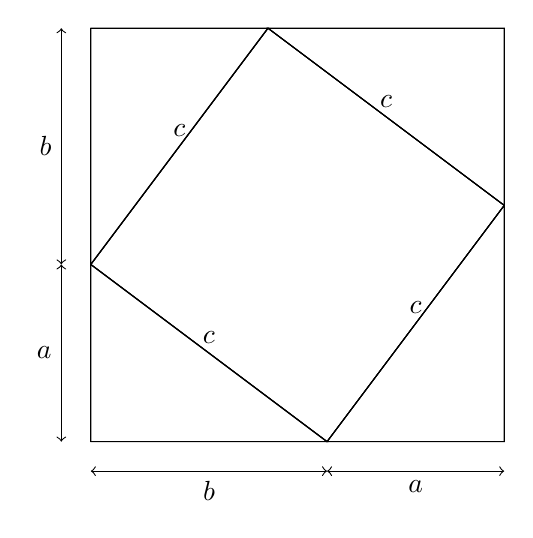
\begin{tikzpicture}[scale=0.75]
    % 辺の長さの定義
    \def\a{3}
    \def\b{4}
    \def\c{5}

    % 大きな正方形の描画
    \draw (0,0) rectangle (\a+\b,\a+\b);

    % 4つの直角三角形の描画
    % 第1の三角形
    \draw (0,0) -- (\b,0) -- (0,\a) -- cycle;
    \draw (0,\a) -- node[midway,above] {$c$} (\b,0);

    % 第2の三角形
    \draw (\b,0) -- (\a+\b,0) -- (\a+\b,\b) -- cycle;
    \draw (\a+\b,\b) -- node[midway,above] {$c$} (\b,0);

    % 第3の三角形
    \draw (\a+\b,\b) -- (\a+\b,\a+\b) -- (\a,\a+\b) -- cycle;
    \draw (\a,\a+\b) -- node[midway,above] {$c$} (\a+\b,\b);

    % 第4の三角形
    \draw (\a, \a+\b) -- (0, \a+\b) -- (0,\a) -- cycle;
    \draw (0,\a) -- node[midway,above] {$c$} (\a, \a+\b);

    % 中央の小さな正方形の描画
    \draw (\b,0) -- (\a+\b,\b) -- (\a,\a+\b) -- (0,\a) -- cycle;

    % 寸法のラベル
    \draw [<->] (-0.5,0) -- (-0.5,\a) node[midway,left] {$a$};
    \draw [<->] (-0.5,\a) -- (-0.5,\a+\b) node[midway,left] {$b$};
    \draw [<->] (0,-0.5) -- (\b,-0.5) node[midway,below] {$b$};
    \draw [<->] (\b,-0.5) -- (\a+\b,-0.5) node[midway,below] {$a$};

  \end{tikzpicture}
\end{example}


\begin{mycolumn}
  証明を記述する際には,文末に$\square$や$\blacksquare$を記すことが一般的である.そのほかに``Q.E.D.''\footnote{``quod erat demonstrandum''の略で,ラテン語で「証明されるべきことでありつづけたこと」という意味である.}などの表現も用いられる.
\end{mycolumn}

\phantomsection
\subsection{命題の反証と反例}

数学において,「すべての$n$に対して$P(n)$が成り立つ」という全称命題が偽であることを証明するには,\textbf{反例}を一つ示すだけで十分である.これは,全称命題が「すべての場合において成り立つ」ことを主張しているため,一つでも例外があれば命題全体が偽となるからである.

\phantomsection
\begin{example}{反例による反証}{反例による反証}
  次の命題を考える:
  \[
    \forall n \in \mathbb{N}\, : \, \frac{n^3}{24} + 84 \geq n^2.
  \]
  この命題が成り立たないことを示すためには,ある$n$について不等式が成立しないことを示せばよい.実際に,$n = 15$のとき,
  \[
    \frac{15^3}{24} + 84 = \frac{3375}{24} + 84 = 140.625 + 84 = 224.625.
  \]
  一方,
  \[
    15^2 = 225.
  \]
  したがって,
  \[
    \frac{15^3}{24} + 84 = 224.625 < 225 = 15^2.
  \]
  このように,$n = 15$において不等式が成り立たないため,元の命題は偽であることが分かる.
\end{example}

また,全称命題が偽であることを証明する際には,「反例をどう見つけたか」ということは明記しない場合が多い.
たとえば\exref{反例による反証}の場合に$n=15$を見つけるには,微分法を用いて議論したり様々な方法があるが,そのような「反例を見つけるまでの過程」を説明する必要はなく,「$n=15$の場合に命題が成り立たないこと」のみを証明として書けばよい.

\phantomsection
\subsection{様々な証明法}

\begin{description}
  \item[帰納法\index{きのうほう@帰納法}] \mbox{} \\
        たとえば数学的帰納法は,数学的な主張が自然数全体に対して成り立つことを示すための証明法である.
  \item[背理法\index{はいりほう@背理法}] \mbox{} \\
        「$P$が成り立たないと仮定すると矛盾が生じる」という論理的な構造を用いて証明を行う方法である.
  \item[直接証明\index{ちょくせつしょうめい@直接証明}] \mbox{} \\
        「$P$が成り立つことを示す」という形式で証明を行う方法である.
\end{description}

以下では,「$n \geq 2$ をみたす任意の自然数について,$2^n > n$である」という命題を3通りのやり方で証明してみよう.

\phantomsection
\begin{example}{帰納法}{帰納法}
  \begin{enumerate}[(I)]
    \item $n=2$のとき,
          \[
            2^2 = 4 > 2
          \]

          となり,与えられた不等式は成立する.
    \item 自然数$k$を$k \geqq 2$を満たすように任意にとる.$2^k > k$ が成り立つと仮定する.このとき,
          \[
            2^{k+1} = 2 \cdot 2^k > 2k.
          \]
          ここで,$k \geqq 2$であるから,$2k - (k + 1) = k - 1 \geq 1$であるがゆえに,$2k > k + 1$である.

          したがって,

          \[
            2^{k+1} > 2k > k + 1.
          \]
          ゆえに,$n=k+1$のときも$2^{k+1} > k + 1$である.
  \end{enumerate}

  以上の考察と数学的帰納法により,$2^n > n$ は $n \geq 2$をみたすすべての自然数について成り立つ.\qed
\end{example}

\phantomsection
\begin{example}{背理法}{背理法}
  $n \geqq 2$をみたす自然数で $2^n \leqq n$ となるものが存在すると仮定する.
  $2^n$ の正の約数の個数は,指数に $1$ を加えたものなので,$2^n$の正の約数の個数は $n + 1$ 個以上である.
  しかし,仮定より $2^n \leqq n$ なので,$2^n$ は $n$ 以下の数である.

  これは,$n$ 以下の数が $n + 1$ 個以上の正の約数を持つことを意味するが,これは矛盾である.

  したがって,先の仮定が誤りであるため,背理法によって$2^n > n$ が成り立つ.\qed
\end{example}

\phantomsection
\begin{example}{直接証明}{直接証明}
  \[
    2^n = n \int_{1}^{2} x^{n-1} \, dx + 1
  \]
  となることはよい.さて,$x \in [1, 2]$ かつ $n \geqq 2$ なので,
  \[
    x^{n-1} \geqq x^{1} \geqq 1
  \]
  が成り立つ.したがって,
  \begin{align*}
    2^n & = n \int_{1}^{2} x^{n-1} \, dx + 1 \\
        & \geqq  n \int_{1}^{2} \, dx +1     \\
        & = n+1.
  \end{align*}
  これと$n+1 >n$であることを併せると,$n \geqq 2$のとき$2^n > n$である.\qed
\end{example}